%%%%%%%%%%%%%%%%%%%%%%%%%%%%%%%%%%%%%%%%%
% Wenneker Assignment
% LaTeX Template
% Version 2.0 (12/1/2019)
%
% This template originates from:
% http://www.LaTeXTemplates.com
%
% Authors:
% Vel (vel@LaTeXTemplates.com)
% Frits Wenneker
%
% License:
% CC BY-NC-SA 3.0 (http://creativecommons.org/licenses/by-nc-sa/3.0/)
% 
%%%%%%%%%%%%%%%%%%%%%%%%%%%%%%%%%%%%%%%%%

%----------------------------------------------------------------------------------------
%	PACKAGES AND OTHER DOCUMENT CONFIGURATIONS
%----------------------------------------------------------------------------------------

\documentclass[11pt]{scrartcl} % Font size

%%%%%%%%%%%%%%%%%%%%%%%%%%%%%%%%%%%%%%%%%
% Wenneker Assignment
% Structure Specification File
% Version 2.0 (12/1/2019)
%
% This template originates from:
% http://www.LaTeXTemplates.com
%
% Authors:
% Vel (vel@LaTeXTemplates.com)
% Frits Wenneker
%
% License:
% CC BY-NC-SA 3.0 (http://creativecommons.org/licenses/by-nc-sa/3.0/)
% 
%%%%%%%%%%%%%%%%%%%%%%%%%%%%%%%%%%%%%%%%%

%----------------------------------------------------------------------------------------
%	PACKAGES AND OTHER DOCUMENT CONFIGURATIONS
%----------------------------------------------------------------------------------------

\usepackage{amsmath, amsfonts, amsthm} % Math packages

\usepackage{listings} % Code listings, with syntax highlighting

\usepackage[english]{babel} % English language hyphenation

\usepackage{graphicx} % Required for inserting images
\graphicspath{{Figures/}{./}} % Specifies where to look for included images (trailing slash required)

\usepackage{booktabs} % Required for better horizontal rules in tables

\numberwithin{equation}{section} % Number equations within sections (i.e. 1.1, 1.2, 2.1, 2.2 instead of 1, 2, 3, 4)
\numberwithin{figure}{section} % Number figures within sections (i.e. 1.1, 1.2, 2.1, 2.2 instead of 1, 2, 3, 4)
\numberwithin{table}{section} % Number tables within sections (i.e. 1.1, 1.2, 2.1, 2.2 instead of 1, 2, 3, 4)

\setlength\parindent{0pt} % Removes all indentation from paragraphs

\usepackage{enumitem} % Required for list customisation
\setlist{noitemsep} % No spacing between list items

%----------------------------------------------------------------------------------------
%	DOCUMENT MARGINS
%----------------------------------------------------------------------------------------

\usepackage{geometry} % Required for adjusting page dimensions and margins

\geometry{
	paper=a4paper, % Paper size, change to letterpaper for US letter size
	top=2.5cm, % Top margin
	bottom=3cm, % Bottom margin
	left=3cm, % Left margin
	right=3cm, % Right margin
	headheight=0.75cm, % Header height
	footskip=1.5cm, % Space from the bottom margin to the baseline of the footer
	headsep=0.75cm, % Space from the top margin to the baseline of the header
	%showframe, % Uncomment to show how the type block is set on the page
}

%----------------------------------------------------------------------------------------
%	FONTS
%----------------------------------------------------------------------------------------

\usepackage[utf8]{inputenc} % Required for inputting international characters
\usepackage[T1]{fontenc} % Use 8-bit encoding

\usepackage{fourier} % Use the Adobe Utopia font for the document

%----------------------------------------------------------------------------------------
%	SECTION TITLES
%----------------------------------------------------------------------------------------

\usepackage{sectsty} % Allows customising section commands

\sectionfont{\vspace{6pt}\centering\normalfont\scshape} % \section{} styling
\subsectionfont{\normalfont\bfseries} % \subsection{} styling
\subsubsectionfont{\normalfont\itshape} % \subsubsection{} styling
\paragraphfont{\normalfont\scshape} % \paragraph{} styling

%----------------------------------------------------------------------------------------
%	HEADERS AND FOOTERS
%----------------------------------------------------------------------------------------

\usepackage{scrlayer-scrpage} % Required for customising headers and footers

\ohead*{} % Right header
\ihead*{} % Left header
\chead*{} % Centre header

\ofoot*{} % Right footer
\ifoot*{} % Left footer
\cfoot*{\pagemark} % Centre footer
 % Include the file specifying the document structure and custom commands

%----------------------------------------------------------------------------------------
%	TITLE SECTION
%----------------------------------------------------------------------------------------

\title{	
	\normalfont\normalsize
	\textsc{\Huge Physics-1 Lab SM203P}\\ % Your university, school and/or department name(s)
	\vspace{25pt} % Whitespace
	\rule{\linewidth}{0.5pt}\\ % Thin top horizontal rule
	\vspace{20pt} % Whitespace
	{\huge Experiment 1: Calculation of the acceleration due to gravity using a
bouncing ball & finding the coefficient of restitution}\\ % The assignment title
	\vspace{12pt} % Whitespace
	\rule{\linewidth}{2pt}\\ % Thick bottom horizontal rule
	\vspace{12pt} % Whitespace
}

\author{\Huge Group-16\\
\\
\LARGE Mayank Chadha(IMT2020045)\\
\\
\LARGE Anshul Jindal(IMT2020039)\\
\\
\LARGE Rahul Jain(IMT2020117)\\
\\
\LARGE Karanjit Saha(IMT2020003)\\
\\
\LARGE Chinmay Parekh(IMT2020069)\\
\\
\LARGE Shashank Shekhar(IMT2020112)} % Your name

\date{\normalsize\today} % Today's date (\today) or a custom date

\begin{document}

\maketitle % Print the title
%----------------------------------------------------------------------------------------
%	FIGURE EXAMPLE
%----------------------------------------------------------------------------------------

\begin{figure}[h] % [h] forces the figure to be output where it is defined in the code (it suppresses floating)
	\centering
	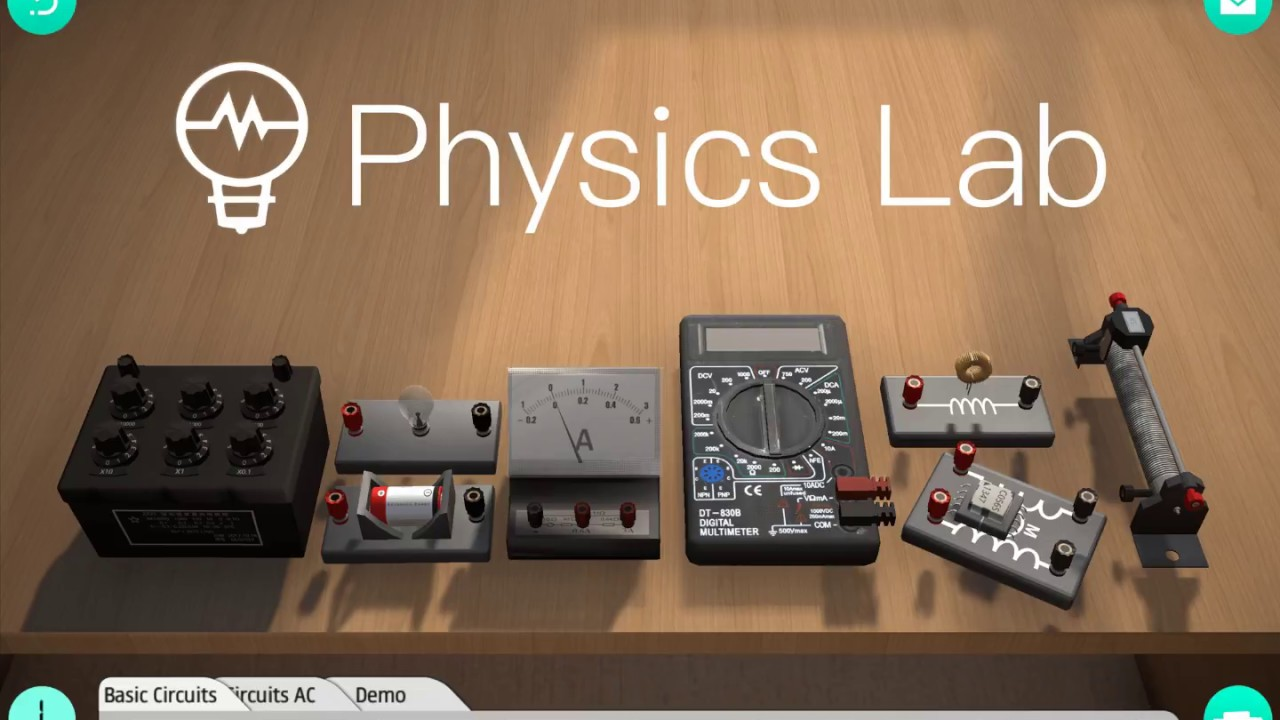
\includegraphics[width=\textwidth, height=5cm]{first.jpg} % Example image
	\caption{Physics lab.}
\end{figure}

%------------------------------------------------
\section{Aim of Experiment}
Calculating the value of acceleration due to gravity (g) at a place and using it to determine the coefficient of restitution (e) between the ball and the ground. \par

\section{Apparatus required for the Experiment}
\begin{enumerate}
	\item Metre scale 
	\item Phyphox mobile app
	\item Ball 
\end{enumerate}





%----------------------------------------------------------------------------------------
%	TEXT EXAMPLE
%----------------------------------------------------------------------------------------

%------------------------------------------------
\section{Theory}
Every experiment uses some or the other instrument to make several measurements, and none of them is perfect. Every instrument has some error associated with it. These errors can be broadly classified into two types, namely systematic errors and random errors.\par 
\textbf{Systematic errors}: - The errors are caused due to imperfect measurement techniques or imperfect apparatus. \\
\textbf{Random errors}: - The errors in measurement are caused by factors that vary from one measurement to another. \par 

Since obliterating these errors is impossible in real-life scenarios. Hence we need to measure how accurate our obtained result is, precisely what we do in error analysis. For doing error analysis, we first need to comprehend the two critical definitions, which are as mentioned below: - \par 

\textbf{A) Accuracy}: - The closeness of the result (or the practical values) to the theoretically calculated values is represented by this quantity. The more accurate our experiment is, the closer is the practical value to the theoretical value.\par

\textbf{B) Precision}: - Precision represents the closeness of the different results obtained by repeating the same experiments in the same situation along with the same apparatus. \par

\subsection{Coefficient of Restitution(e)}
From the definition of the coefficient of restitution we know, 
\begin{align} 
	\begin{split}
		e = \frac{h_1}{h_0}\\
	\end{split}					
\end{align}

%------------------------------------------------
\subsubsection{Procedure (for calculating e)}
For finding e, we follow the below-mentioned steps: - \par

A) Release the ball from some height ‘$h_0$’ and note it in the observation table. \par

B) Record the height to which the ball rises after the first collision (let it be ‘$h_1$’) and note it in the observation table. \par

C) Calculate e by using the equation mentioned beforehand. \par

D) Repeat the above steps several times to get a good idea about the actual e and fill the observation table accordingly. \par

E) Calculate the average of all the e’s calculated in the above steps. This e is the coefficient of restitution of the ball. \par

\subsubsection{Errors (for e)}
The equation deduced after error analysis on the above equation is:\par
Derivation for the Error Propagation:
\begin{align} 
		e &= \frac{h_1}{h_0} \nonumber
\end{align}
Taking log both sides :
\begin{align}
\log_e e &= \log_e h_1 + \log_e h_0 \nonumber
\end{align}
   Finally we get:
\begin{align} 
	\begin{split}
		\frac{\partial{e}}{e} &= \frac{\partial{h_1}}{h_1} + \frac{\partial{h_0}}{h_0}\\
	\end{split}					
\end{align}

\subsection{Acceleration Due to Gravity(g)}

\begin{figure*}
    \centering
    \includegraphics[width=9cm,height=7cm]{fig.PNG}
    \caption{Schematic representation of bounces of ball. Note that ball should not have any horizontal component of velocity.}
    \label{fig:my_label}
\end{figure*}\n

As we know from Newton’s motion of equations, that if an object is dropped (i.e., initial velocity =0) from some height ‘h’ (such that h is negligibly small compared to the radius of the earth), then  \par

\begin{align} 
	\begin{split}
		h &= \frac{1}{2}gt^2\\
	\end{split}					
\end{align}

where g = acceleration due to gravity and t= time taken for the object to reach the ground. \par

\subsubsection{Procedure (for calculating g)}
For finding g, we follow the below-mentioned steps: - \par

A) Select a random number ‘n’ such that the ball will be able to bounce at least n number of times. Also, select a height $h_0$ (which will be constant throughout the experiment)\par

B) Drop the ball from $h_0$ height, record the total time it takes to do n bounces, and name it $t_n^*$. \par

C) Fill the below mentioned observation table and use the formula mentioned below to use the previously fetched e and the respective $h_0$ and $t_n^*$ to calculate g. \par\par

Derivation of the formula for calculating g:\par



Let $t_1$ be the time taken between $1^{st}$ and $2^{nd}$ bounce\par
$t_2$ be the time taken between $2^{nd}$ and $3^{rd}$ bounce and so on...\par\par
Let total time be $t_n^*$\par and let ball be dropped from initial height $h_0$.

\par
Modifying Equation 3.1, we get:\par
\begin{align} 
	\begin{split}
		h &= \frac{2h_1}{(\frac{t_1}{2})^2}=\frac{8h_0e}{(t_1)^2}\\
	\end{split}					
\end{align}

Now we know that:\par
\begin{align} 
	\begin{split}
		 t_n^*=t_1+t_2+t_3 +....+ t_n \\
	\end{split}					
\end{align}

From equation 3.1 we get:\par


\begin{align} 
	\begin{split}
		 t_n^*=t_1+2\sqrt{\frac{2h_2}{g}}+2\sqrt{\frac{2h_3}{g}}+....+2\sqrt{\frac{2h_n}{g}}\\
	\end{split}					
\end{align}

Substituting value of e in equation 3.3, we get:\par

\begin{align} 
	\begin{split}
		 t_n^*=t_1+2(\frac{t_1}{2})\sqrt{e}+2(\frac{t_1}{2})\sqrt[3]{e}+....+2(\frac{t_1}{2})\sqrt[n]{e}\\
	\end{split}					
\end{align}

Taking common terms out and applying sum of G.P:\par
\begin{align} 
	\begin{split}
		 t_1=\frac{t_n^*(\sqrt{e}-1)}{(\sqrt{e})^n-1}\\
	\end{split}					
\end{align}

Substituting $t_1$ from equation 3.6 in equation 3.2, we finally get:\par
\begin{align} 
	\begin{split}
		\boxed{g = \frac{8h_0e}{t_{n}^{*2}}\left(\dfrac{(\sqrt{e})^n-1}{\sqrt{e}-1}\right)^2}\\
	\end{split}					
\end{align}
	 
D) The final value of g will be the avg of all the g’s obtained in the experiment. \par

\subsubsection{Errors (for g)}
The equation deduced after error analysis on the above equation is:(Assuming n=3)\par
\textbf{Least count for heights h and $h_0$ = 0.01 m and for time = 0.001 s.}\par

Derivation for the Error Propagation:
\begin{align} 
		g &= \frac{8h_0e}{t_{n}^{*2}}\left(\dfrac{(\sqrt{e})^n-1}{\sqrt{e}-1}\right)^2 \nonumber
\end{align}
    Taking logarithmic on both sides and taking n = 3:
\begin{align} 
            \log_e g &= \log_e h_0 + \log_e t^{-2} + 2(log_e ({e^{3/2}-1}) - log_e ({\sqrt{e}-1})) \nonumber
\end{align}
    Differentiating on both sides we get:
\begin{align} 
        \frac{\partial{g}}{g} &= \frac{\partial{h_0}}{h_0} + \frac{\partial{e}}{e} + \frac{2\partial{t_n^*}}{t_n^*} + \left|\frac{3\partial{e^{3/2-1}}}{\sqrt{e}-1} + \frac{\partial{e^{-1/2}}}{\sqrt{e}-1}\right|\partial{e} \nonumber
\end{align}
   On further solving the above equation we get:
\begin{align} 
	\begin{split}
		\boxed{\frac{\partial{g}}{g} = \frac{\partial{h_0}}{h_0} + \frac{\partial{e}}{e}+\frac{2\partial{t_m^*}}{t_m^*}+\left|\frac{3\sqrt{e}\partial{e}}{e^{3/2}-1}\right|+\left|\frac{\partial{e}}{\sqrt{e}(\sqrt{e}-1)}\right|}\\
	\end{split}					
\end{align}
%------------------------------------------------



\section{Sources of Error}
\begin{enumerate}
	\item Air Resistance
	\item Inclined or Rough Surface
	\item Parallax error while measuring the height of the ball from ground
	\item Phyphox mobile app uses various sensors which are present in a mobile phone, which may not give accurate results every time.
	\item Random error.
\end{enumerate}
%----------------------------------------------------------------------------------------
%	EQUATION EXAMPLES
%----------------------------------------------------------------------------------------
\newpage

\section{Observation and Calculation}
\subsection{Mayank Chadha(IMT2020045)}
\begin{figure}[h] % [h] forces the figure to be output where it is defined in the code (it suppresses floating)
	\centering
	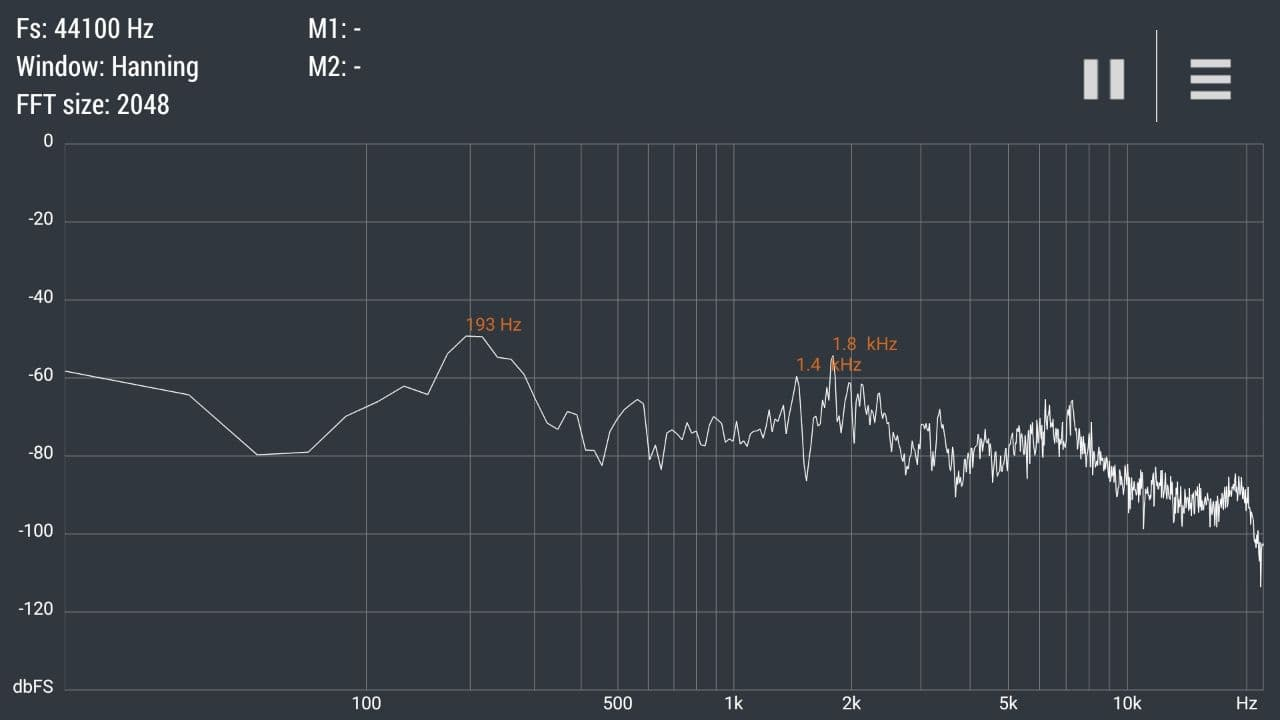
\includegraphics[width=12cm, height=8cm]{700ml.jpg} % Example image
	\caption {Plot given by Advanced Spectrum Analyzer}
\end{figure}
Volume of the cavity taken is 0.7 L.\par
Peak Frequency according to graph generated is 193 Hz.\par
Area of the neck was approximately 0.133 m.\par
Effective length of neck = 0.19 m.\par
Therefore, by calculation we get speed of sound(c) =324.08



\end{document}
